\documentclass{beamer} 
\usetheme{default} 
\setbeamercovered{transparent}

%\useoutertheme{umbcfootline} 
\setbeamertemplate{background canvas}[vertical shading][bottom=red!20,top=yellow!30] 


\usepackage[spanish]{babel}
%\usepackage[latin1]{inputenc}
\usepackage[utf8x]{inputenc}
\usepackage{multicol}


\title{Archivos binarios}

\author{Manuel J. Molino Milla \and Luis Molina Garzón}

\date{\today} %

\institute{IES Virgen del Carmen \and Departamento de Informática}




%\beamerdefaultoverlayspecification{<+->}

\begin{document}


\begin{frame}
  \titlepage
\end{frame}

\begin{frame}
    \frametitle{Logo}
\begin{figure}

\includegraphics[scale=1]{imagenes/logo.jpeg} 
\caption{Logo Java}
\end{figure}
\end{frame}

\begin{frame}
  \frametitle{Contenido}
 \tableofcontents[pausesections]
\end{frame}



\subsection{Introduccion}
\begin{frame}[fragile]
\frametitle{Ficheros binarios}
\begin{footnotesize}
\begin{itemize}[<+->]
\item Los ficheros binarios almecenan datos en binario.
\item Son diseñados para ser leídos por programas.
\item Ejemplo: los ficheros fuentes de java son almacenados en ficheros de texto, pero los ficheros compilados se almacenan en binario.
\item Los ficheros binarios son mas eficientes a la hora de procesarlos.
\item Ejemplo el número 199 se almacena en un fichero de texto como una secuencia de caracteres 1-9-9 y en un binario como \emph{C7} su equivalente en hexadecimal.
\item Recordamos que para leer y escribir ficheros de texto, creamos objetos de la clase \emph{Scanner} y \emph{PrintWriter}
\item Ejemplo:
\end{itemize}
\begin{verbatim}
PrintWriter output = new PrintWriter("temp.txt");
output.print("Java 101");
output.close();
.....
Scanner input = new Scanner(new File("temp.txt"));
System.out.println(input.nextLine());
\end{verbatim}
\end{footnotesize}
\end{frame}

\begin{frame}
\frametitle{Ficheros}
\begin{itemize}[<+->]
\item Los computadores no diferencia entre ficheros de texto y binario.
\item Todos los ficheros son almacenados de forma binaria.
\item Las I/O de texto están construidas sobre I/O binarias, mediante un nivel de abstracción añadida.
\item Quiere decir que cuando guardamos texto en un fichero se codifica y para la lectura se descodifican.
\item En cambio para los datos binarios este paso no hace falta hacerlo.
\item De ahí la mayor eficiencia en las operaciones I/O en binario
\end{itemize} 
\end{frame}

\subsection{Clases I/O binario}
\begin{frame}
\frametitle{InputStream y OutputStream} 
\begin{figure}
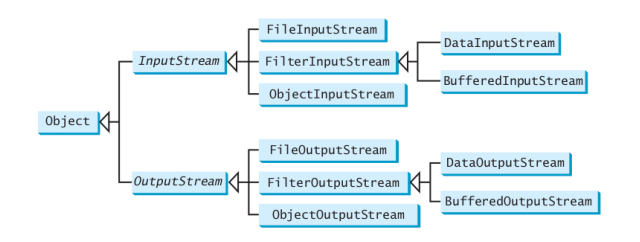
\includegraphics[scale=0.6]{imagenes/io.png} 
\caption{InputStream y OutputStream}
\end{figure} 
\end{frame}

\subsection{InputStream}
\begin{frame}
\frametitle{InputStream} 
\begin{multicols}{2}
\begin{figure}
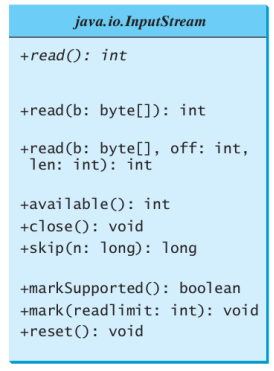
\includegraphics[scale=0.5]{imagenes/input.png} 
%\caption{InputStream y OutputStream}
\end{figure} 
\begin{footnotesize}
\begin{itemize}[<+->]
\item Lee el siguiente byte de un \emph{inputstream}, el valor devuelto está entre 0 y 255. Si no lee un byte devuelve \emph{-1}
\item Lee b.length() bytes y devuelve el número de bytes leídos. Devuelve \emph{-1} si es el final del stream.
\item Lee bytes desde b[off], b[off+1], \dots ,b[off+len-1]. Devuelve el número de bytes leido; \emph{-1} si llega al final.
\item Devuelve el número de bytes que pueden ser leidos.
\item Cierra el input stream
\item Hace un salto en el stream y descarta los mismos.
\item Comprueba si el stream soporta los métodos \emph{mark()} y \emph{reset}
\item Marca la posición del input stream.
\item Reposiciona la posición del stream y eliminas las marcas realizadas 
\end{itemize}
\end{footnotesize}
\end{multicols}
\end{frame}


\subsection{OutputStream}
\begin{frame}
\frametitle{OutputStream} 
\begin{multicols}{2}
\begin{figure}
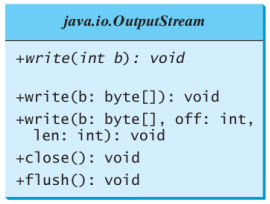
\includegraphics[scale=0.7]{imagenes/out.png} 
%\caption{InputStream y OutputStream}
\end{figure} 
\begin{itemize}[<+->]
\item Escribe el byte en le stream como (byte)b.
\item Escribe todos los bytes especificados.
\item Escribe los bytes b[off], b[off+1], \dots ,b[off+len-1].
\item Vuelca los bytes al fichero de salida.
\end{itemize}
\end{multicols}
\end{frame}


\subsection{FileInputStream y FileOutputStream}
\begin{frame}
\frametitle{FileInputStream y FileOutputStream} 
\begin{multicols}{2}
\begin{figure}
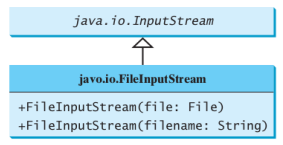
\includegraphics[scale=0.6]{imagenes/fi.png} 
%\caption{InputStream y OutputStream}
\end{figure}
\begin{figure}
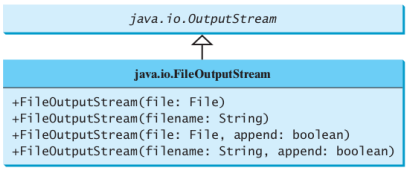
\includegraphics[scale=0.45]{imagenes/fo.png} 
%\caption{InputStream y OutputStream}
\end{figure} 
\begin{itemize}[<+->]
\item Si append esta a true los datos serán añadidos al fichero.
%\item Evitando que se sobreescriba.
\item La mayoría de los métodos de I/O requieren \emph{java.io.IOException}
\end{itemize}
\end{multicols}
\end{frame}

\begin{frame}[fragile]
\frametitle{Ejemplo}
\begin{scriptsize}
\begin{verbatim}
import java.io.*;
public class TestFileStream
{
  public static void main (String[]args) throws IOException
  {
// Create an output stream to the file
    FileOutputStream output = new FileOutputStream ("temp.dat");
// Output values to the file
    for (int i = 1; i <= 10; i++)
        output.write (i);
// Close the output stream
      output.close ();
// Create an input stream for the file
    FileInputStream input = new FileInputStream ("temp.dat");
// Read values from the file
    int value;
    while ((value = input.read ()) != -1)
      System.out.print (value + " ");
// Close the output stream
      input.close ();
      System.out.println ();
  }
}
\end{verbatim}
\end{scriptsize}
\end{frame}

\subsection{FilterInputStream/FilterOutputStream}

\begin{frame}
\frametitle{FilterInputStream/FilterOutputStream}
\begin{itemize}[<+->]
\item Son clases que nos facilitan la escritura y lectura de datos.
\item Están diseñadas para lectura/escritura de \emph{int, double y string}
\item Para todos los datos primitivos usamos las clases \emph{DataInputStream y DataOutputStream}
\end{itemize}
\end{frame}



\subsection{DataInputStream/DataOutputStream}
\begin{frame}
\frametitle{DataInputStream/DataOutputStream}
\begin{multicols}{2} 
\begin{figure}
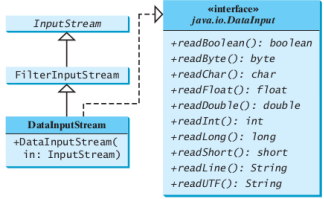
\includegraphics[scale=0.6]{imagenes/di.png} 
\end{figure} 
\begin{figure}
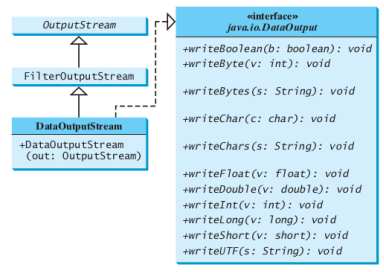
\includegraphics[scale=0.5]{imagenes/do.png} 
\end{figure}
\end{multicols}
\end{frame}

\begin{frame}[fragile]
\frametitle{Ejemplo}
\begin{tiny}
\begin{verbatim}
import java.io.*;
public class TestDataStream
{
  public static void main (String[]args) throws IOException
  {
// Create an output stream for file temp.dat
    DataOutputStream output =
      new DataOutputStream (new FileOutputStream ("temp.dat"));
// Write student test scores to the file
      output.writeUTF ("John");
      output.writeDouble (85.5);
      output.writeUTF ("Jim");
      output.writeDouble (185.5);
      output.writeUTF ("George");
      output.writeDouble (105.25);
// Close output stream
      output.close ();
// Create an input stream for file temp.dat
    DataInputStream input =
      new DataInputStream (new FileInputStream ("temp.dat"));
// Read student test scores from the
      System.out.println (input.readUTF () + " " + input.readDouble ());
      System.out.println (input.readUTF () + " " + input.readDouble ());
      System.out.println (input.readUTF () + " " + input.readDouble ());
  }
}
\end{verbatim}
\end{tiny}
\end{frame}

\begin{frame}[fragile]
\frametitle{Detectanto final de fichero}
\begin{tiny}
\begin{verbatim}
import java.io.*;
public class DetectEndOfFile
{
  public static void main (String[]args)
  {
    try
    {
      DataOutputStream output = new DataOutputStream
        (new FileOutputStream ("test.dat"));
        output.writeDouble (4.5);
        output.writeDouble (43.25);
        output.writeDouble (3.2);
        output.close ();
      DataInputStream input = new DataInputStream
        (new FileInputStream ("test.dat"));
      while (true)
        {
          System.out.println (input.readDouble ());
        }
    }
    catch (EOFException ex)
    {
      System.out.println ("All data read");
    }
    catch (IOException ex)
    {
      ex.printStackTrace ();
    }
  }
}
\end{verbatim}
\end{tiny}
\end{frame}

\subsection{BufferedInputStream/BufferedOutputStream}

\begin{frame}[fragile]
\frametitle{BufferedInputStream/BufferedOutputStream}
\begin{itemize}[<+->]
\item Son clases que hacen que la escritura y lectura de datos sea más rápida.
\item Estas clases no contienen métodos.
\item Usa los métodos heredados de \emph{InputStream/OutputStream}
\item Si no se usa el tamaño del buffer su valor por defecto es \emph{512 bytes}
\item Ejemplo:
\end{itemize}
\begin{verbatim}
DataOutputStream output = new DataOutputStream(
new BufferedOutputStream (new FileOutputStream("temp.dat")));
DataInputStream input = new DataInputStream(
new BufferedInputStream (new FileInputStream("temp.dat")));
\end{verbatim}
\end{frame}

\begin{frame}[fragile]
\frametitle{BufferedInputStream/BufferedOutputStream}
\begin{figure}
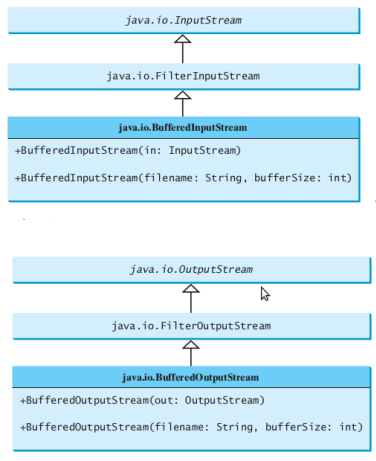
\includegraphics[scale=0.7]{imagenes/buffer.png} 
\caption{Lenguaje máquina}
\end{figure} 
\end{frame}

\begin{frame}[fragile]
\frametitle{Ejemplo}
\begin{tiny}
\begin{verbatim}
import java.io.*;
public class Copy{
//args[0] for sourcefile args[1] for target file
  public static void main (String[]args) throws IOException  {
// Check command-line parameter usage
    if (args.length != 2)
      { System.exit (0); }
// Check whether source file exists
    File sourceFile = new File (args[0]);
    if (!sourceFile.exists ())
      {
        System.out.println ("Source file " + args[0] + " not exist");
        System.exit (0);
      }
// Check whether target file exists
    File targetFile = new File (args[1]);
    if (targetFile.exists ())
      { System.out.println ("Target file " + args[1] + " already exists");
        System.exit (0); }
// Create an input stream
    BufferedInputStream input = new BufferedInputStream (new FileInputStream(sourceFile));
// Create an output stream
    BufferedOutputStream output =new BufferedOutputStream (new FileOutputStream(targetFile));
// Continuously read a byte from input and write it to output
    int r;int numberOfBytesCopied = 0;
    while ((r = input.read ()) != -1)
      {output.write ((byte) r);
        numberOfBytesCopied++; }
// Close streams
    input.close ();output.close ();
// Display the file size
    System.out.println (numberOfBytesCopied + " bytes copied");
  }
}
\end{verbatim}
\end{tiny}
\end{frame}

\subsection{ObjectInputStream/ObjectOutputStream}

\begin{frame}[fragile]
\frametitle{ObjectInputStream/ObjectOutputStream}
\begin{itemize}[<+->]
\item DataInputStream/DataOutputStream nos proporciona una interfaz para datos primitivos y String.
\item \emph{ObjectInputStream/ObjectOutputStream} nos proporciona una interfaz para cualquier tipo de objetos.
\end{itemize}
\begin{figure}
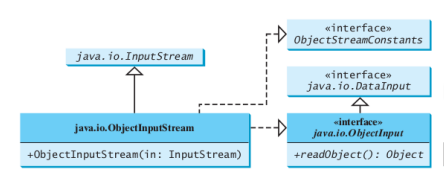
\includegraphics[scale=0.5]{imagenes/is.png}
\end{figure}
\begin{figure}
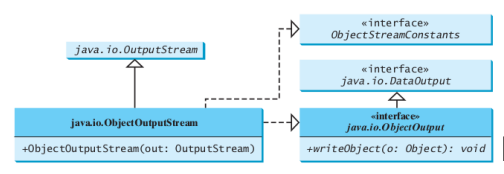
\includegraphics[scale=0.5]{imagenes/os.png}
\end{figure}
\end{frame}

\begin{frame}[fragile]
\frametitle{Ejemplo}
\begin{tiny}
\begin{verbatim}
import java.io.*;
public class TestObjectOutputStream
{
  public static void main (String[]args) throws IOException
  {
// Create an output stream for file object.dat
    ObjectOutputStream output =
      new ObjectOutputStream (new FileOutputStream ("object.dat"));
// Write a string, double value, and object to the file
      output.writeUTF ("John");
      output.writeDouble (85.5);
      output.writeObject (new java.util.Date ());
// Close output stream
      output.close ();
  }
}
\end{verbatim}
\begin{verbatim}
import java.io.*;
public class TestObjectInputStream
{
  public static void main (String[]args) throws ClassNotFoundException,
    IOException
  {
// Create an input stream for file object.dat
    ObjectInputStream input =
      new ObjectInputStream (new FileInputStream ("object.dat"));
// Write a string, double value, and object to the file
    String name = input.readUTF ();
    double score = input.readDouble ();
      java.util.Date date = (java.util.Date) (input.readObject ());
      System.out.println (name + " " + score + " " + date);
// Close output stream
      input.close ();
  }
}
\end{verbatim}
\end{tiny}
\end{frame}

\subsection{Serialización de un objeto}

\begin{frame}[fragile]
\frametitle{Serialización de un objeto}
\begin{itemize}[<+->]
\item Se llama''serializar un objeto'' al proceso de convertirlo a bytes, para poder enviarlo por una red, y reconstruirlo luego a partir de esos bytes.
\item Para que un programa java pueda convertir un objeto en un montón de bytes y pueda luego recuperarlo, el objeto necesita ser \emph{Serializable}. 
\item Al poder convertir el objeto a bytes, ese objeto se puede enviar a través de red, guardarlo en un fichero.
\item Después se puede reconstruir el objeto al otra lado de la red, leerlo del fichero,\dots
\item Para que un objeto sea serializable basta con que implemente la interfaz Serializable.
\item Como la interfaz Serializable no tiene métodos, es muy sencillo implementarla.
\item Basta con un \alert{implements Serializable} y nada más.
\end{itemize}
\end{frame}

\begin{frame}[fragile]
\frametitle{Ejemplo}
\begin{verbatim}
public class Datos implements Serializable
{
   public int a;
   public String b;
   public char c;
}
\end{verbatim}
\begin{verbatim}
public class DatoGordo implements Serializable
{
   public int d;
   public Integer e;
   Datos f;
}
\end{verbatim}
\end{frame}

\begin{frame}
\frametitle{Serialización de arrays}
\begin{itemize}[<+->]
\item Un array es serializable si todos sus componentes son serializables.
\item Podemos usar para serializar objetos, la clase \emph{ObjectOutputStream} y para deserializarlos la clase \emph{ObjectInputStream}
\item Un array se puede serializar usando el método \alert{writeObject}.
\item Y se puede recuperar con posteriormente usando \alert{readObject}
\end{itemize}
\end{frame}

\begin{frame}[fragile]
\frametitle{Ejemplo}
\begin{tiny}
\begin{verbatim}
import java.io.*;
public class TestObjectStreamForArray
{
  public static void main (String[]args) throws ClassNotFoundException,
    IOException
  {
    int[] numbers = { 1, 2, 3, 4, 5 };
      String[] strings = {"John", "Jim", "Jake"};
// Create an output stream for file array.dat
    ObjectOutputStream output =
      new ObjectOutputStream (new FileOutputStream ("array.dat", true));
// Write arrays to the object output stream
    output.writeObject (numbers);
    output.writeObject (strings);
// Close the stream
    output.close ();
// Create an input stream for file array.dat
    ObjectInputStream input =
      new ObjectInputStream (new FileInputStream ("array.dat"));
    int[] newNumbers = (int[]) (input.readObject ());
    String[]newStrings = (String[])(input.readObject ());
// Display arrays
    for (int i = 0; i < newNumbers.length; i++)
      System.out.print (newNumbers[i] + " ");
    System.out.println ();
    for (int i = 0; i < newStrings.length; i++)
      System.out.print (newStrings[i] + " ");
  }
}
\end{verbatim}
\end{tiny}
\end{frame}



\subsection{Ficheros de acceso aleatorio}

\begin{frame}[fragile]
\frametitle{Ficheros de acceso aleatorio}
\begin{itemize}[<+->]
\item Todos los \emph{stream} que hemos visto hasta ahora son de solo-escritura o solo-lectura.
\item Son ficheros secuenciales que no pueden ser actualizados sin la creación de un nuevo fichero.
\item A menudo es necesario modificar ficheros, por ejemplo añadiendo nuevos datos.
\item Java posee la clase \alert{RandomAccessFile} que permite a un fichero ser de lectura y escrituro con accesos aleatorios.
\item \emph{RandomAccessFile} implementa las interfaces \alert{DataInput} y \alert{DataOutput}
\item DataInput define los siguientes métodos: \alert{readInt, readDouble, readChar, readBoolean, readUTF}
\item DataOutput define: \alert{writeInt, writeDouble, writeChar, writeBoolean, writeUTF}.
\end{itemize}
\end{frame}

\begin{frame}
\frametitle{Constructor}
\begin{itemize}[<+->]
\item RandomAccessFile(file: File, mode: String) 
\item RandomAccessFile(name: String, mode: String) 
\item Se puede construir a partir de un objeto File o a partir del objeto String que indica la ruta del fichero.
\item El modo a especificar es ''r'' o ''rw'', que indica que es de solo lectura o lectura o escritura.
\item Ejemplo: \emph{RandomAccessFile raf = new RandomAccessFile(''test.dat'',''"rw'');}
\item Si el fichero existe se abre para acceso aleatorio, sino se crea y se prepara para dicho acceso.
\item \alert{raf.close()} cierra el stream.
\item \alert{raf.length()} nos da el número de bytes que tiene el fichero.
\end{itemize}
\end{frame}

\begin{frame}
\frametitle{Características de los accesos aleatorios}
\begin{itemize}[<+->]
\item Un fichero de acceso aleatorio es una secuencia de bytes.
\item Una marca especial denominada \alert{puntero de fichero} se coloca en uno de los bytes.
\item Cuando se abre un fichero se posiciona al principio.
\item Cuando se leen o escriben bytes el puntero se mueve.
\item Ejemplo si leemos un entero (4 bytes) el puntero se desplaza 4 bytes.
\item \alert{raf.seek(position)} mueve el puntero a una posición determinada.
\item \alert{raf.length()} nos da el número de bytes que tiene el fichero.
\end{itemize}
\begin{figure}
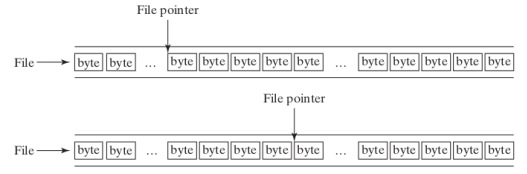
\includegraphics[scale=0.4]{imagenes/puntero.png}
\end{figure}
\end{frame}

\begin{frame}
\frametitle{Otros métodos de RandomAccessFile}
\begin{itemize}
\item \alert{getFilePointer(): long} devuelve el \emph{offset} en bytes desde el principio del fichero a donde va a suceder la siguiente lectura o escritura.
\item \alert{read(b: byte[]): int} lee b.length bytes
\item \alert{setLength(newLength: long): void} establece una nueva longitud para el fichero.
\item \alert{skipBytes(int n): int} salta n bytes en la entrada.
\end{itemize}
\end{frame}

\begin{frame}[fragile]
\frametitle{Ejemplo}
\begin{tiny}
\begin{verbatim}
import java.io.*;
public class TestRandomAccessFile{
  public static void main (String[]args) throws IOException  {
// Create a random-access file
    RandomAccessFile inout = new RandomAccessFile ("inout.dat", "rw");
// Clear the file to destroy the old contents, if any
      inout.setLength (0);
// Write new integers to the file
    for (int i = 0; i < 200; i++)
        inout.writeInt (i);
// Display the current length of the file
      System.out.println ("Current file length is " + inout.length ());
// Retrieve the first number
      inout.seek (0);           // Move the file pointer to the beginning
      System.out.println ("The first number is " + inout.readInt ());
// Retrieve the second number
      inout.seek (1 * 4);       // Move the file pointer to the second number
      System.out.println ("The second number is " + inout.readInt ());
// Retrieve the tenth number
      inout.seek (9 * 4);       // Move the file pointer to the tenth number
      System.out.println ("The tenth number is " + inout.readInt ());
// Modify the eleventh number
      inout.writeInt (555);
// Append a new number
      inout.seek (inout.length ());     // Move the file pointer to the end
      inout.writeInt (999);
// Display the new length
      System.out.println ("The new length is " + inout.length ());
// Retrieve the new eleventh number
      inout.seek (10 * 4);      // Move the file pointer to the next number
      System.out.println ("The eleventh number is " + inout.readInt ());
      inout.close ();
  }
}
\end{verbatim}
\end{tiny}
\end{frame}

\begin{frame}
\frametitle{Preguntas} 
\begin{figure}

\includegraphics[scale=0.9]{imagenes/dudas.png} 
\caption{Lenguaje máquina}
\end{figure} 
\end{frame}

\end{document}

